\documentclass[10pt,a4paper]{article}
\usepackage[italian]{babel}
\usepackage[T1]{fontenc}
\usepackage[utf8]{inputenc}
\usepackage[affil-it]{authblk}
\usepackage{lineno,hyperref}
\usepackage{amsmath}
\usepackage{amsfonts}
\usepackage{amssymb}
\usepackage{graphicx}
\usepackage{subcaption}


\newtheorem{remark}{Osservazione}
\newtheorem{definition}{Definizione}
\newtheorem{theorem}{Teorema}

\newcommand{\ww}{\mathbf{w}}
\newcommand{\vv}{\mathbf{v}}
\newcommand{\ee}{\mathbf{e}}
\newcommand{\ii}{\mathbf{i}}
\newcommand{\oo}{\mathbf{o}}

\begin{document}
\title{Appunti di Artificial Intelligence}

\author{Ivan Masnari%
  \thanks{e-mail: \texttt{ivan.masnari@studenti.unimi.it}}}
\affil{Facoltà di Informatica, UniMi, Milano}

\date{Ultima modifica: \today}
\maketitle
\section{Introduzione}

Dato un qualunque sistema, se disponiamo di un insieme di leggi o regole che lo descrivono completamente (nel caso di un sistema fisico avremmo delle equazioni differenziali) potremmo, in teoria, calcolarne in ogni momento lo stato e, quindi, prevederne l'evoluzione nel tempo. 
Tuttavia, nella vita di ogni giorno capita spesso di non avere a disposizione una conoscenza perfetta di un certo sistema. Tale informazione:
\begin{enumerate}
\item{può mancare.}
\item{possiamo averne una conoscenza approssimata.}
\end{enumerate}
L'intelligenza artificiale nasce con lo scopo di estrarre conoscenza direttamente dai dati in nostro possesso attraverso strumenti automatici. Questo modello si differenzia rispetto alla descrizione \emph{a priori} del sistema, in quanto lo simula per comprenderne \emph{a posteriori} il suo comportamento. Per far questo, è stato utile studiare come gli esseri viventi interagiscano con l'ambiente circostante e come vi si adattino.
Vari modelli di intelligenza artificiale sono stati proposti lungo la storia della disciplina. Una categorizzazione preliminare che si fa in letteratura è quella tra modelli:
\begin{itemize}
\item{\emph{simbolici}, in cui i dati vengono sottoposti a codifica e solo dopo manipolati. Storicamente questo è stato il primo approccio adottato (vedi sistemi esperti degli anni '70).}
\item{\emph{pre-simbolici}, in cui i dati vengono manipolati direttamente, senza la mediazione di una codifica. Fanno parte di questa famiglia: le reti neurali, i sistemi fuzzy e gli algoritmi evolutivi.}
\end{itemize}
Nel corso ci concentreremo sui secondi.

\section{Reti neurali}

\subsection{Background biologico}

Il nostro cervello ci permette di analizzare in maniera molto sofisticata l'ambiente in cui ci troviamo per agire nel miglior modo possibile (esempio: se riconosciamo un leone nella savana, scappiamo nell'altra direzione). Queste analisi sono basate sul funzionamento del cervello: come estrae informazioni, come queste interagiscono con l'informazioni contenute in memoria, etc. Lo studio di questi processi è un campo di ricerca molto attivo e multidisciplinare dove convergono gli interessi della biologia, della medicina e della psicologia.
Tali studi ci offrono dei modelli che simulano l'attività celebrale. Proprio questi modelli, vengono poi utilizzati dall'informatica per offrire strumenti di predizione, ottimizzazione e problem-solving in vari campi applicativi (guida automatizzata, smart cities, etc.). Il successo di questi modelli è condizionato dal fatto che il nostro cervello è un potente computer capace di computare in parallelo grandi porzioni di dati. Ma come funziona esattamente?

\begin{figure}
\centering
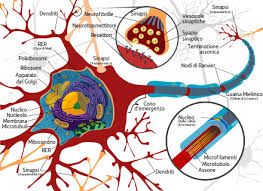
\includegraphics[scale=0.7]{img/neurone.jpeg}
\caption{Neurone}
\label{fig:1}
\end{figure}

Il cervello è composto da miliardi di cellule dette \emph{neuroni} (Figura \ref{fig:1}). Il neurone a sua volta è costituito da:
\begin{itemize}
\item{i \emph{dendriti}, i quali sono filamenti raggiunti dalle terminazioni di altri neuroni e che gli permettono di raccogliere informazioni grazie a processi biochimici originati dai così detti \emph{neurotrasmettitori}.}
\item{l'\emph{assone}: un lungo filamento che parte dal corpo centrale della cellula e trasmette segnali elettrici che, a loro volta, vanno ad attivare altri neuroni attraverso il rilascio di neurotrasmettitori.}
\end{itemize}

Quando e come il neurone trasmetta il segnale di attivazione dipende dal particolare modello fisiologico che si voglia adottare. Solitamente si considera un \emph{threshold}, superato il quale, l'assone viene depolarizzato e la differenza di potenziale provoca il passaggio di una corrente. Un diverso modello prende in considerazione non tanto la potenza dello stimolo quanto il loro numero. 
Questa struttura a network offre ottime prestazioni. Per un confronto con una CPU classica alleghiamo la seguente tabella:

\begin{figure}
\centering
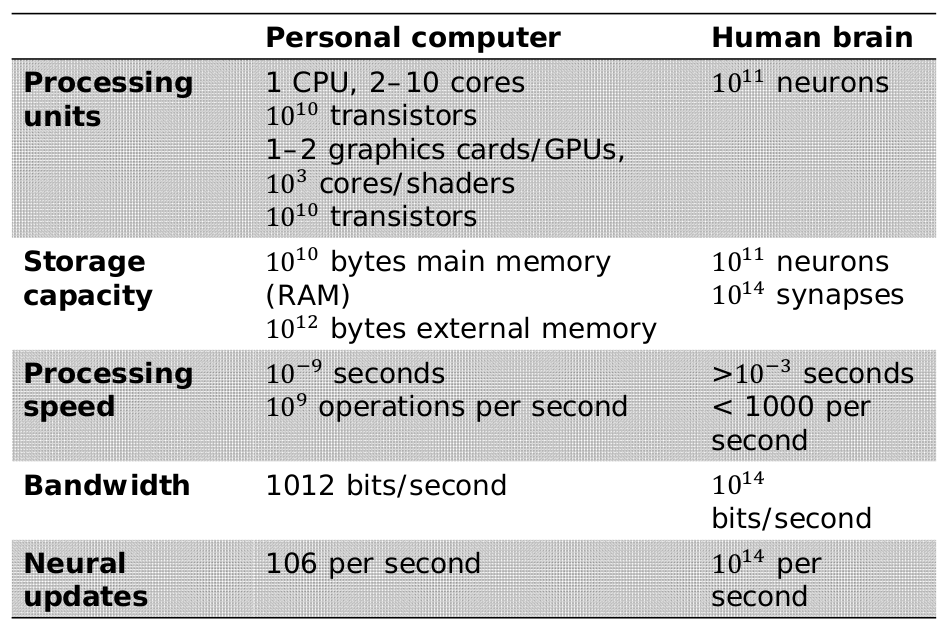
\includegraphics[scale=0.3]{img/cpuvshuman.png}
\end{figure}

\newpage

I vantaggi delle reti neurali sono:

\begin{enumerate}
\item{Alta velocità di calcolo, grazie al parallelismo.}
\item{Tolleranza ai guasti: la rete rimane funzionale anche quando molti neuroni smettono di funzionare.}
\item{La performance degrada in modo lineare con il numero di neuroni danneggiati.}
\item{Ottimo per l'apprendimento induttivo.}
\end{enumerate}

\subsection{Threshold logic unit}

Per implementare una rete neurale artificiale occorre trovare un analogo del neurone naturale. Tale compito è svolto dalle \emph{threshold logic unit}, nel seguito TLU. Una TLU è costituita da $n$ variabili di input $x_1 \dots x_n$ e un output $y$. Ad ogni unità viene assegnato un \emph{threshold} $\theta$ e ad ogni variabile di input un peso $w_i$ dove $i \in \{1, \dots ,n\}$ che rappresenta la rilevanza ai fine della computazione di quel particolare input.
L'output della TLU viene calcolato secondo la seguente formula:

\begin{equation}
y =  \begin{cases}
    1 & \text{se } \sum w_ix_i \geq \theta \\
    0 & \text{altrimenti} 
   \end{cases}
\end{equation}

Attraverso questo semplice meccanismo possiamo simulare alcune funzioni booleane. Se volessimo computare l'AND logico tra due input $x_1$ e $x_2$ basta assegnare valori ai pesi e al threshold in modo che soddisfino il seguente sistema di disequazioni:

\begin{equation}
	\begin{cases}
    w_1 + w_2 \geq \theta \\
    w_1 < \theta\\
    w_2 < \theta
   \end{cases}
\end{equation}

Risulta evidente che l'unica circostanza in cui l'output della TLU verrà posto ad 1 sarà quando entrambi gli input si trovano a 1. Inoltre, si noti che esistono varie scelte possibili di pesi e threshold che verificano le diseguaglianze.

\subsection{Interpretazione geometrica}

La condizione che calcola l'output della TLU somiglia molto da vicino all'equazione di un iperpiano (ovvero, un piano in $n$ dimensioni):

\begin{equation}
	 \sum w_ix_i + \theta = 0 
\end{equation}

Se pensiamo al caso precedente dell'AND logico e consideriamo i valori di input come coordinate in uno spazio bidimensionale, possiamo vedere che la retta definita da $x_1w_1 + x_2w_2 + \theta = 0$ corrisponde al confine che separa quelle combinazioni di valori che restituiscono come output 1 e quelle che, invece, restituiscono 0 (vedi Figura 2). \\
Da quanto detto, tuttavia, si può dedurre che una singola TLU potrà computare solo funzioni \emph{linearmente separabili}, ovvero funzioni in cui le coordinate associate agli input che restituiscono 1 possono essere separate da quelle che restituiscono 0 da una funzione lineare (punto, retta, piano o iperpiano a seconda della dimensione). 

\begin{figure}
\centering
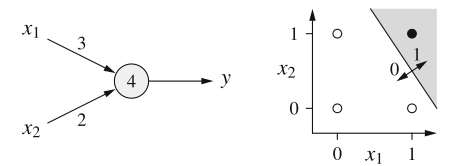
\includegraphics[scale=0.5]{img/geometria.png}
\caption{Rappresentazione geometrica della TLU per $x_1 \land x_2$}
\label{fig:2}
\end{figure}

\begin{definition}
Un insieme di punti $X$ in uno spazio euclideo si dice \emph{convesso} se e solo se non è vuoto, è connesso e ogni coppia di punti può essere congiunta da un segmento.
\end{definition}
\begin{definition}
Un \emph{guscio convesso} di un insieme di punti $X$ in uno spazio euclideo è il più piccolo insieme convesso che contiene $X$.
\end{definition}
\begin{theorem}
Due insiemi di punti $X$ e $Y$ si dicono linearmente separabili se e solo se i loro gusci convessi sono tra loro disgiunti.
\end{theorem}

Questo significa che già all'interno delle funzioni booleane ne esistono alcune che non possono essere simulate da una TLU. Come, per esempio, la doppia implicazione. Sebbene solo due funzioni booleane a due argomenti non siano linearmente indipendenti, al crescere degli argomenti il numero di funzioni che sono linearmente indipendenti diminuisce rapidamente. Per un numeri di argomenti arbitrariamente grande, una singola TLU non può calcolare "quasi" nessuna funzione.

\begin{figure}
\centering
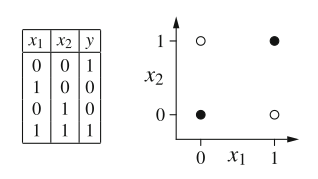
\includegraphics[scale=0.5]{img/doppiaimplicazione.png}
\caption{La doppia implicazione non è linearmente separabile}
\label{fig:3}
\end{figure}

Il problema può essere ovviato attraverso la costruzione di network di TLU più complessi. Come esempio consideriamo il network che simula la doppia implicazione (vedi figura \ref{fig:4}).

\begin{figure}
\centering
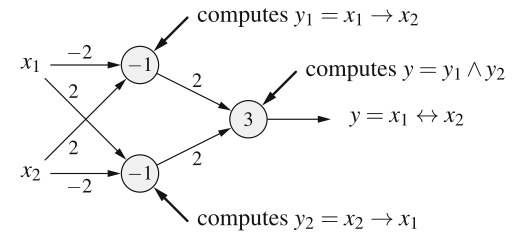
\includegraphics[scale=0.5]{img/netTLU.png}
\caption{network di TLU che simula la doppia implicazione}
\label{fig:4}
\end{figure}

\subsection{Training delle TLU}

L'interpretazione geometrica ci da una intuizione su come costruire una TLU avente 2 o 3 input, ma non è un metodo scalabile, nè automatizzato. Come far evolvere una TLU affinchè converga in modo autonomo ad una soluzione?
Un algoritmo che ci permette di automatizzare il processo è il seguente:

\begin{enumerate}
\item{Inizializzare i pesi e il threshold con valori randomici.}
\item{Determinare l'errore nell'output per un insieme di controlli. L'errore viene calcolato come una funzione dei pesi e del threshold $e(w_1,\dots,w_n,\theta)$.}
\item{Aggiornare i pesi e il threshold per correggere l'errore.}
\item{Iterare finchè l'errore si annulla.}
\end{enumerate}

Mostriamo il comportamento dell'algoritmo nel caso più semplice, in cui abbiamo un threshold ed un unico input (quindi, un unico peso associato). Poniamo che si voglia allenare il nostro neurone a calcolare la negazione booleana. Sia $x$ l'input, $w$ il peso associato e $\theta$ il threshold, allora l'output $y$ sarà definito come:

\begin{equation}
	y = \begin{cases}
    1 & \text{se } 0w = 0 \geq \theta \\
    0 & \text{se } 1w = w \geq \theta
   \end{cases}
\end{equation} 

Calcoliamo la funzione errore al variare di $w$ e $\theta$. Nel caso che $x = 0$ l'errore sarà 0 per un $\theta$ negativo e 1 per un $\theta$ negativo. Il peso non avrà alcuna influenza perchè viene annullato nella moltiplicazione con l'input. Quando, invece, $x = 1$, avremo che la funzione dipenderà da entrambi i parametri (vedi Figura \ref{fig:5}).

\begin{figure}
\centering
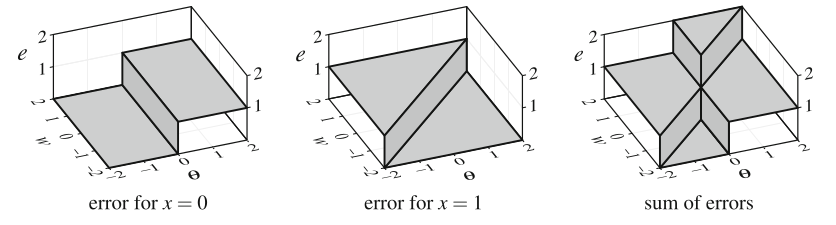
\includegraphics[scale=0.4]{img/error1.png}
\caption{funzione di errore per la negazione booleana}
\label{fig:5}
\end{figure}

La funzione di errore così calcolata non può essere usata direttamente nella nostra computazione perchè è composta da plateau e, quindi, non è ovunque derivabile. La soluzione è quella di calcolare la funzione di errore in modo tale che ci offra una misura di "quanto sbagliata" sia la relazione tra pesi e threshold. Otterremo così una funzione di errore che, seppur ancora non differenziabile, (vedi Figura \ref{fig:6}) lo sia localmente nei punti in cui l'errore si discosta da $0$. Ciò che faremo per correggere l'errore, dunque, sarà discendere verso l'area dove la funzione di errore si annulla. Questo è possibile esattamente perché abbiamo costruito una funzione derivabile nei punti in cui ci interessa, e cioè possiamo sempre calcolare la direzione migliore da prendere perchè si "scenda".
Ci sono due modi di immaginare il processo di allenamento del neurone:

\begin{itemize}
\item{\emph{Online learning}: dove correggiamo l'errore individualmente per ogni scelta dell'input.}
\item{\emph{Batch learning}: dove prendiamo in considerazione l'errore cumulato su una sequenza di input prima di applicare le correzioni.}
\end{itemize}

\begin{figure}
\centering
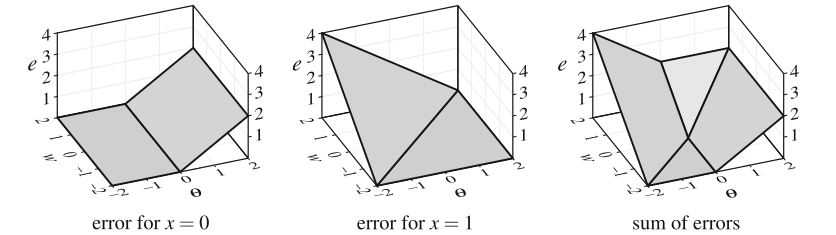
\includegraphics[scale=0.4]{img/error2.png}
\caption{funzione di errore differenziabile}
\label{fig:6}
\end{figure}

Definiamo di seguito la \emph{delta rule} o \emph{procedura di Widrow-Hoff} per allenare le TLU:

\begin{definition}
Sia $\vv$ = ($x_1, \dots, x_n$) il vettore di input di una TLU, \emph{o} l'output aspettato e \emph{y} il valore attuale. Se \emph{o} = \emph{y}, abbiamo finito. Al contrario, per ridurre l'errore computeremo nuovi valori per il threshold e i pesi nel seguente modo:
$$
\theta^{(new)} = \theta^{(old)} + \Delta\theta \text{ con } \Delta\theta = -\eta(\emph{o} - \emph{y})
$$
$$
\forall i \in \{1, \dots, n\}:w_i^{(new)} = w_i^{(old)} + \Delta w_i \text{ con } \Delta w_i = \eta(\emph{o} - \emph{y})x_i
$$
dove $\eta$ è il \emph{learning rate}. Più è alto, più i cambiamenti sui pesi e sui threshold sono drastici.

\end{definition}

Abbiamo visto prima, tuttavia, che non tutte le funzioni possono essere computate. Per le funzioni linearmente separabili esiste un teorema che ci garantisce che applicando la \emph{delta rule} l'algoritmo converga ad una soluzione.

\begin{theorem}
Sia $L = \{(\vv_1,\emph{o}_1), \dots, (\vv_n,\emph{o}_n)\}$ una sequenza di pattern di allenamento per la TLU, dove $\vv_i$ sono i vettori di input e $\emph{o}_i$ l'output atteso. 
Siano inoltre $L_0 = \{(\vv,\emph{o}) \in L | \emph{o} = 0\}$ e $L_1 = \{(\vv,\emph{o}) \in L | \emph{o} = 1\}$ rispettivamente gli insiemi delle coppie di pattern che hanno come output atteso 0 e quelle che hanno come pattern atteso 1. Se $L_0$ e $L_1$ sono linearmente separabili, allora esiste un $\ww$ vettore di pesi e un $\theta$ threshold t.c.:
$$
\forall (\vv,0) \in L_0: \ww\vv < \theta 
$$
$$
\forall (\vv,1) \in L_1: \ww\vv \geq \theta
$$
\end{theorem}

\begin{remark}
Negli esempi precedenti abbiamo codificato il valore booleano \emph{falso} come 0 e \emph{vero} come 1. Questa scelta ha lo svantaggio che, nel caso di \emph{falso}, i pesi corrispondenti non possano essere modificati perchè la formula contiene l'input come fattore. Per evitare il problema si ricorre in letteratura ad una diversa codifica chiamata \emph{ADALINE} (ADAptive LINear Element), dove \emph{falso} viene ad assumere il valore $-1$ e il \emph{vero} $1$.
\end{remark}

Notiamo che questa procedura di allenamento vale solo per le singole TLU, ma abbiamo prima visto che le TLU possono computare solo funzioni linearmente separabili. Sebbene questo inconveniente si possa evitare prendendo in esame \emph{network} di TLU, questa procedura non si estende naturalmente a quel caso.

\subsection{Artificial neural network}

Un artificial neural network (in quello che segue ANN) può essere rappresentata come un grafo diretto $G = (U,C)$ dove i nodi sono TLU e gli archi sono le connessioni tra le varie unità. L'insieme dei nodi $U$ può essere partizionato in tre sottoinsiemi:

\begin{itemize}
\item{$U_{(in)}$: è l'insieme dei nodi di input, i quali ricevono in modo diretto l'informazione dall'ambiente.}
\item{$U_{(out)}$: è l'insieme dei nodi di output, i quali sono i soli nodi a comunicare con l'esterno.}
\item{$U_{(hidden)}$: è l'insieme dei nodi interni, i quali propagano la computazione.}
\end{itemize}

\begin{figure}
\centering
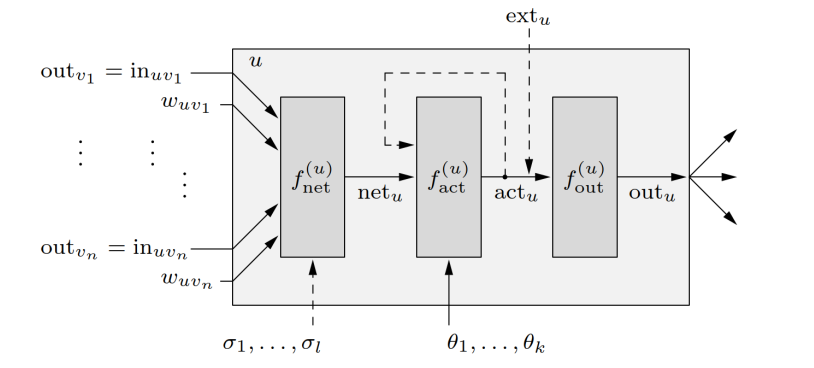
\includegraphics[scale=0.4]{img/ANN.png}
\caption{rappresentazione di un singolo neurone}
\label{fig:7}
\end{figure}

Ogni connessione $(u,v) \in C$ possiede un peso $w_{uv}$ che definisce l'importanza del dato originato da $v$ per il neurone $u$. Ad ogni neurone $u \in U$ vengono, invece, assegnate quattro variabili: il \emph{network input} $net_u$, la \emph{activation} $act_u$, l'\emph{output} $out_u$ e l'\emph{external input} $ext_u$ (vedi Figura \ref{fig:7}). Le prime tre variabili vengono calcolate in ogni momento dell'evoluzione dell'ANN grazie a tre funzioni associate:

\begin{enumerate}
\item{La \emph{network input function} $f^u_{net}$: calcola la somma pesata dell'input.}
\item{La \emph{activation function} $f^u_{act}$: ne esistono vari modelli (gaussiana, sigmoide, etc.) a seconda dell'applicazione.}
\item{La \emph{output function} $f^u_{out}$: definisce l'output a seconda che il neurone venga o meno attivato.}
\end{enumerate}

Se il grafo che rappresenta l'ANN è aciclico si parla di \emph{feed forward network} e la computazione procede in modo unidirezionale da $U_{(in)}$ a $U_{(out)}$ seguendo l'ordine topologico\footnote{L'ordine topologico è una numerazione dei vertici di un grafo diretto tale che tutti gli archi partano da un nodo associato ad un numero minore rispetto a quello associato al nodo di arrivo. Un ordine topologico esiste solo per grafi aciclici.} del network. Nel caso, invece, il grafo contenga un ciclo, allora si parla di \emph{recurrent network}.
I processi all'interno di un ANN si dividono in due fasi:

\begin{enumerate}
\item{La \emph{input phase}: dove gli input esterni vengono acquisiti dai neuroni di input.}
\item{La \emph{work phase}: dove i neuroni di input vengono spenti e un nuovo output viene computato da ogni neurone. La \emph{work phase} continua finchè gli output sono stabili o si raggiunge un timeout.}
\end{enumerate}

\begin{figure}
\centering
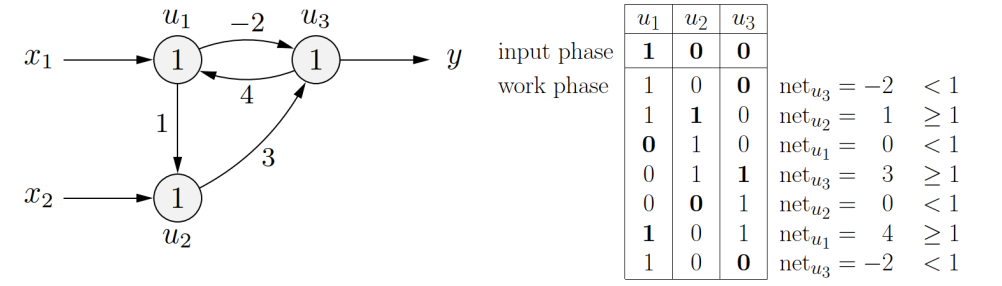
\includegraphics[scale=0.3]{img/rnn1.png}
\caption{computazione di una recurrent neural network che non giunge ad uno stato stabile}
\label{fig:8}
\end{figure}


Nel caso delle recurrent neural network, potrebbe accadere che non si giunga mai ad uno stato stabile a seconda di quale ordine di update dei neuroni si scelga di seguire. In Figura \ref{fig:8} abbiamo un esempio di una computazione con risultato oscillante in un recurrent neural network. L'ordine seguito per l'update è: $u_3,u_1,u_2,u_3,u_1,u_2\dots$. Se si fosse seguito un diverso ordine la computazione avrebbe raggiunto uno stato stabile.

\subsection{Training delle ANN}

Abbiamo visto in precedenza che è possibile allenare in modo automatico una singola TLU grazie alla delta rule. Come abbiamo già avuto modo di osservare questo procedimento non può essere generalizzato alle ANN. Tuttavia, i principi a cui ci ispiriamo sono i medesimi: calcolare correzioni ai pesi ed ai threshold dei singoli neuroni e aggiornarli di conseguenza. A seconda del tipo dei dati che utilizziamo per allenare le nostre ANN e dei criteri di ottimizzazione distiguiamo due tipi di apprendimento:

\begin{enumerate}
\item{\emph{fixed learning task} o apprendimento con supervisione}
\item{\emph{free learning task} o apprendimento senza supervisione}
\end{enumerate}

Nel caso di una fixed learning task avremo un insieme 
$L=\{(\ii_1,\oo_1),\dots,(\ii_n,\oo_n)\}$ di coppie che assegnano ad ogni input un output desiderato. Una volta completato il processo di apprendimento, la ANN dovrebbe essere in grado di restituire l'output adeguato rispetto all'input che le viene presentato. In pratica, questo accade raramente e bisogna accontentarsi di un risultato approssimativo.
Per giudicare in che misura una ANN si avvicina alla soluzione della fixed learning task si adotta una funzione di errore. Solitamente tale funziona viene calcolata come il quadrato della differenza tra l'output desiderato e quello attuale:
$$
e = \sum_{l \in L} \sum_{v \in U_{(out)}} e^l_v
$$
dove
$$
e^l_v = (o^l_v - out_v)^2
$$
è l'errore individuale per una particolare coppia $l$ e un neurone di output $v$. Il quadrato delle differenze viene scelto per vari motivi. Per prima cosa, errori positivi e negativi altrimenti si cancellerebbero a vicenda e non sarebbero presi in considerazione. In secondo luogo, questa funzione è ovunque derivabile, semplificando così il processo di aggiornamento dei pesi e dei threshold.
Nel free learning task avremo, invece, solo una sequenza di input $L = \{\ii_1, \dots, \ii_n\}$. Questo comporta che, a differenza del fixed learning task, non avremo modo di calcolare una funzione di errore rispetto ad un output atteso. In linea di principio, infatti, l'obiettivo di un free learning task sarà quello di produrre un output "simile" per input "simili". Un caso particolare potrebbe essere quello del \emph{clustering} dei vettori di input. 
Qualsiasi processo di apprendimento si scelga esistono alcune buone pratiche che è utile seguire. Una è quella di normalizzare il vettore di input. Comunemente lo si scala in modo tale che abbia media uguale a 0 e la varianza ad 1. Per fare questo uno deve calcolare per ogni neurone $u_k \in U_{(in)}$ la media aritmetica $\mu_k$ e la deviazione standard $\sigma_k$ degli input esterni:

$$
\mu_k = \frac{1}{|L|}\sum_{l \in L} ext^l_{u_k} \quad \quad \sigma_k = \sqrt{\frac{1}{|L|}\sum_{l \in L} (ext^l_{u_k} - \mu_k)^2}
$$

Quindi gli input esterni vengono ricalcolati secondo questa formula:

$$
ext^{new}_{u_k} = \frac{ext^{old}_{u_k} - \mu_k}{\sigma_k}
$$

\subsection{Multi-layer perceptrons}

\begin{figure}
\centering
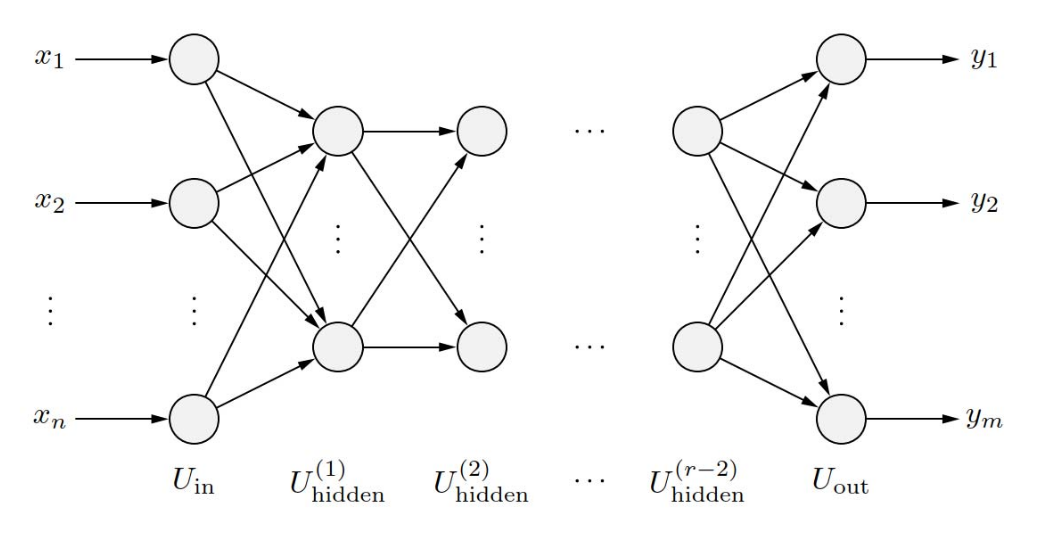
\includegraphics[scale=0.3]{img/MLP.png}
\caption{multi-layer perceptrons}
\label{fig:9}
\end{figure}


Una delle prime ANN sviluppate furono i \emph{multi-layer perceptrons} (nel seguito MLP). Le MLP sono particolari feed-forward network  in cui le unità base (i percettroni) sono organizzati in \emph{layer} e ogni layer ha connessioni solo con il layer successivo (vedi Figura \ref{fig:9}). Questo permette di minimizzare il fenomeno delle continue ricomputazioni che avverrebbero durante la propagazione del segnale nei normali feed-forward network.
La network input function di ogni neurone $u \in U_{(hidden) \cup U_{(out)}}$ viene calcolata come la somma pesata degli input, come:
$$
f^u_{net}(\ww_u,\ii_u) = \sum_{v \in pred(u)} w_{uv}out_v
$$
L'activation function, invece, è una così detta \emph{funzione sigmoide}, ossia una funzione monotona non descrescente tale che:
$$
f: \mathbb{R} \to [0,1] \quad \text{ con } \lim_{x\to-\infty}f(x) = 0 \quad \text{ e } \lim_{x\to\infty}f(x) = 1
$$

\begin{figure}

\begin{subfigure}{0.5\textwidth}
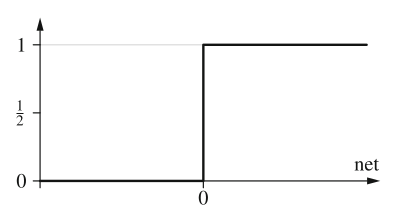
\includegraphics[width=0.9\linewidth, height=3cm]{img/step.png} 
\caption{step function}
\end{subfigure} %%
\begin{subfigure}{0.5\textwidth}
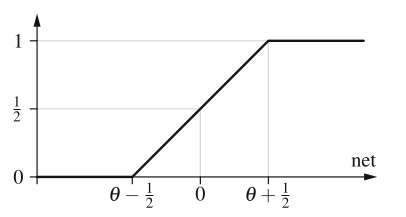
\includegraphics[width=0.9\linewidth, height=3cm]{img/semilinear.png}
\caption{semi-linear function}
\end{subfigure} 
\begin{subfigure}{0.5\textwidth}
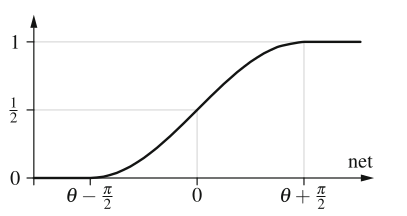
\includegraphics[width=0.9\linewidth, height=3cm]{img/sineup.png} 
\caption{sine up to saturation}
\end{subfigure}
\begin{subfigure}{0.5\textwidth}
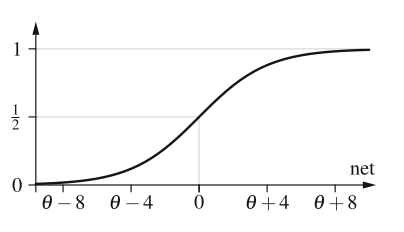
\includegraphics[width=0.9\linewidth, height=3cm]{img/logistic.png} 
\caption{logistic function}
\end{subfigure}


\caption{Alcune funzioni sigmoidi}
\label{fig:10}
\end{figure}

La funzione di output può essere sia una sigmoide oppure una semplice funzione lineare. \\
La struttura a layer di un MLP suggerisce che si possa descrivere il network con l'aiuto di una matrice dei pesi. In questo modo la computazione del MLP può essere rappresentata attraverso la moltiplicazione tra matrici e vettori. Tuttavia, noi non abbiamo utilizzato in classe una matrice per l'intero network, ma una per ogni singolo layer. Siano $U_1 = \{ v_1, \dots, v_n \}$ e $U_2 = \{ u_1, \dots, u_m \}$ due layer consecutivi di neuroni. I pesi delle loro connessioni sono codificati in una matrice $W$ di dimensioni $n \times m$:

$$
W = \begin{pmatrix}
  w_{u_1v_1} & w_{u_1v_2} & \cdots & w_{u_1v_n} \\
  w_{u_2v_1} & w_{u_2v_2} & \cdots & w_{u_2v_n} \\
  \vdots  & \vdots  & \ddots & \vdots  \\
  w_{u_mv_1} & w_{u_mv_2} & \cdots & w_{u_mv_n} 
 \end{pmatrix}
$$

Se due neuroni $u_i$ e $v_j$ non sono connessi, è sufficiente porre $w_{u_iv_j} = 0$. Il vantaggio di questa matrice sta nel fatto che è possibile scrivere il network input di un layer come:

$$
\mathbf{net}_{U_2} = W \mathbf{in}_{U_2} = W \mathbf{out}_{U_1}
$$

dove $\mathbf{net}_{U_2} = (net_{u_1}, \dots, net_{u_m})^\top$ e $\mathbf{in}_{U_2} = \mathbf{out}_{U_1} = (out_{v_1}, \dots, out_{v_n})^\top$. \\
Fino ad adesso abbiamo visto che le ANN possono rappresentare funzioni booleane, ma quando si parla di funzioni a valori continui? 


\begin{theorem}
Ogni funzione Riemann-integrabile è approssimata con precisione arbitraria da un MLP avente quattro layer.
\end{theorem}

\begin{figure}
\centering
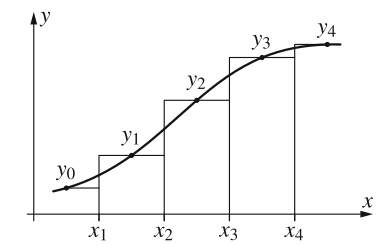
\includegraphics[scale=0.4]{img/approx.png}
\caption{Approssimazione di una funzione continua con una step function}
\label{fig:11}
\end{figure}

\begin{figure}
\centering
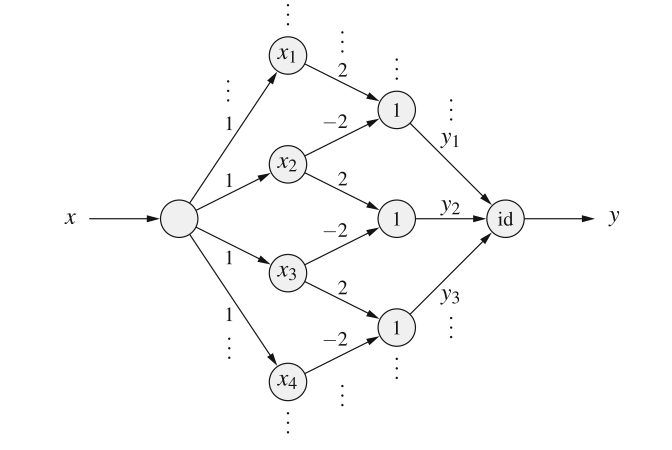
\includegraphics[scale=0.3]{img/riemann.png}
\caption{MLP che calcola la step function in Figura \ref{fig:11}}
\label{fig:12}
\end{figure}

Ogni funzione, infatti, può essere approssimata da una step function (come in Figura \ref{fig:11}). Ad ogni pivot $x_i$ associamo nel nostro MLP un neurone nel primo hidden layer (vedi Figura \ref{fig:12}). Nel secondo hidden layer creiamo un neurone per ogni scalino, il quale riceverà input dai due neuroni del primo livello che sono assegnati ai valori $x_i$ e $x_{i+1}$ che definiscono i bordi dello scalino. A questo punto, scegliamo pesi e threshold in modo tale che il neurone venga attivato se e solo se l'input è maggiore di $x_i$ e minore di $x_{i+1}$. Siccome la funzione di attivazione del neurone di output è la funzione di identità, il valore così calcolato viene emesso così come è ricevuto. 
Dovrebbe essere chiaro che l'approssimazione può crescere a piacere semplicemente aggiungendo neuroni e diminuendo la lunghezza dei gradini. Possiamo, inoltre, risparmiarci un layer se non utilizziamo nel calcolo l'altezza assoluta ma quella relativa come peso della connessione al neurone di output.
Bisogna notare, comunque, che questo risultato non ha natura costruttiva, ossia non ci dice come deve essere fatto un MLP che approssimi con una data accuratezza una certa funzione. Tutto ciò che afferma il Teorema 3 è che limitare il numero di layer non pregiudica la proprietà del MLP di essere un \emph{approssimatore universale}.

\subsection{Regressione}

Abbiamo visto che per allenare un ANN occorre minimizzare la funzione di errore, la quale si calcola solitamente come il quadrato della differenza tra output aspettato e attuale. Questo avvicina il problema dell'apprendimento nelle reti neurali a quello più generale della \emph{regressione}. La regressione è una tecnica molto usata in analisi e in statistica per estrapolare la retta (o, più in generale, il polinomio) che meglio approssima la relazione esistente in un insieme di dati/osservazioni. Detto in modo più formale, se $G = \{(\ww_0,y_0), \dots, (\ww_n,y_n)\}$ è il nostro dataset e immaginiamo esista una relazione funzionale tra il vettore di input $\ww_i$ e l'ascissa $y$, allora la regressione ci aiuterà a trovare i parametri di quella funzione. A seconda del diverso genere di funzione avremo diverse forme di regressione.

\subsubsection{Regressione lineare}

Se ci aspettiamo che le nostre due quantità $x$ e $y$ esibiscano una dipendenza lineare, allora dovremo identificare i parametri $a$ e $b$ che individuano la retta $y = g(x) = a + bx$. In generale, tuttavia, non sarà possibile trovare una singola retta che passi per tutti i punti del nostro dataset. Quello che faremo sarà trovare la retta che devi dai punti il meno possibile e che, quindi, minimizzi l'errore calcolato come segue: 

$$
F(a,b) = \sum(g(x_i) - y_i)^2 = \sum(a + bx_i - y_i)^2
$$

Il teorema di Fermat ci dice che una condizione necessaria perchè un minimo della funzione $F(a,b)$ esista è che la derivata parziale in entrambi i parametri si annulli:

$$
\frac{\partial F}{\partial a} = \sum 2(a + bx_i - y_i) = 0
$$

$$
\frac{\partial F}{\partial b} = \sum 2(a + bx_i - y_i)x_i = 0
$$

Questo sistema può essere risolto con alcune semplici tecniche di algebra lineare (vedi pag. 174 del libro). La soluzione così trovata sarà unica a meno che ogni valore $x_i$ sia identico. 

\subsubsection{Regressione polinomiale e multilineare}

Il metodo precedente può essere esteso in modo ovvio a polinomi di ordine arbitrario. In questo caso, si prende come ipotesi che la funzione indotta dal dataset approssimi un polinomio di ordine $n$:

$$
y = p(x) = a_o + a_1x + \dots + a_nx^n
$$

E si cercherà di minimizzare la funzione $F$ tale che:

$$
F(a_1,\dots,a_n) = \sum(p(x_i) - y_i)^2 = \sum(a_o + a_1x + \dots + a_nx^n -y_i)^2
$$

Come nel caso della regressione lineare, la funzione potrà essere minimizzata solo se le derivate parziali rispetto ai parametri $a_i$ si annullano:

$$
\frac{\partial F}{\partial a_1} = 0 \quad \dots \quad \frac{\partial F}{\partial a_n} = 0
$$

Inoltre, non siamo limitati a calcolare funzioni ad un solo argomento. Con alcune minori modifiche questo metodo è capace di approssimare funzioni in un numero arbitrario di argomenti. In quel caso, la chiameremo \emph{regressione multilineare}.

\subsubsection{Regressione logistica}

Nel situazione in cui il nostro dataset non sia approssimato con sufficiente accuratezza da una funzione polinomiale, potremmo dover utilizzare funzioni di generi diversi. Data, per esempio, una funzione della forma:

$$
y = ax^b
$$

possiamo trasformarla in una equazione lineare applicando l'operazione di logaritmo:

$$
ln(y) = ln(a) + b \cdot ln(x)
$$

Nel caso delle ANN ci interessiamo in particolare alla funzione logistica (vedi Figura \ref{fig:10}(d)):

$$
y = \frac{Y}{1 + e^{a+bx}}
$$

Siccome molte ANN utilizzano come funzione di attivazione del neurone proprio la funzione logistica, se trovassimo un modo di applicarci il metodo della regressione potremmo determinare i parametri di qualsiasi network a due layer con un unico input. Il valore $a$ nella funzione corrisponderebbe al threshold del neurone di output e la $b$ al peso dell'input. Possiamo "linearizzare" la funzione logistica applicandoci le seguenti trasformazioni (comunemente chiamata \emph{logit transformation}):

$$
y = \frac{Y}{1 + e^{a+bx}} \leftrightarrow \frac{1}{y} = \frac{1 + e^{a+bx}}{Y} \leftrightarrow \frac{Y - y}{y} = e^{a+bx} \leftrightarrow ln(\frac{Y - y}{y}) = a+bx
$$

Se estendiamo il nostro approccio fino a comprendere funzioni con più argomenti, in analogia a quanto accade nella regressione multilineare, possiamo utilizzarlo per computare i pesi di network a due layer con arbitrari neuroni di input. Tuttavia, siccome il metodo della somma degli errori funziona solo quando parliamo di neuroni di output, questo approccio non può essere esteso a network con più di due layer.

\subsection{Backpropagation}

Come abbiamo appena visto la regressione logistica funziona solo per MLP con due layer di neuroni. Un approccio più generale è quello del \emph{gradient descent}. Il metodo consiste nell'utilizzare la funzione di errore per calcolare la direzione in cui cambiare i pesi e il threshold per minimizzare l'errore. Condizione necessaria per il suo utilizzo è che la funzione sia differenziabile. Tuttavia, un MLP ha una funzione logistica come funzione di attivazione e, quindi, la funzione di errore sarà differenziabile (posto che la funzione di output sia la funzione identità).
Intuitivamente, il \emph{gradiente} descrive la pendenza di una funzione. Questo è calcolato assegnando ad ogni punto del dominio della funzione un vettore, i cui componenti sono le derivate parziali rispetto ai agli argomenti(un esempio in Figura \ref{fig:13}). L'operazione di calcolare il gradiente (di un punto o di una funzione) è comunemente denotata con l'operatore differenziale $\nabla$ (pronuncia: nabla).

\begin{figure}
\centering
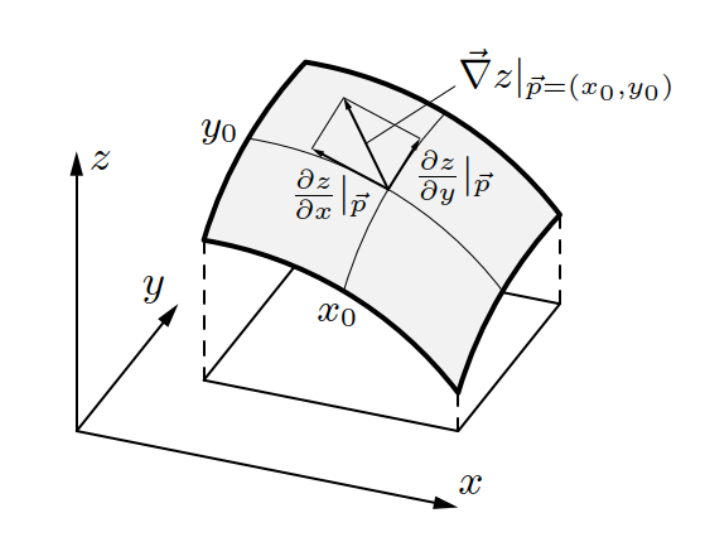
\includegraphics[scale=0.3]{img/gradient.png}
\caption{Il gradiente di una funzione a due argomenti.}
\label{fig:13}
\end{figure}

Nel caso delle MLP, calcolare il gradiente della funzione di errore si traduce nel calcolare la derivata parziale della funzione di errore rispetto ai pesi e i threshold presi come parametri. Sia $\ww_u = (-\theta,w_{u_1},\dots,w_{u_k})$ il vettore dei pesi di un singolo layer esteso così da includere anche il threshold, calcoliamo il gradiente come segue:
$$
\nabla_{\ww_u} e = \frac{\partial e}{\partial \ww_u} = (-\frac{\partial e}{\partial \theta}, \frac{\partial e}{\partial w_{u_1}},\dots,\frac{\partial e}{\partial w_{u_k}})
$$
Siccome l'errore totale $e$ è dato dalla somma degli errori individuali rispetto a tutti i neuroni e tutti i training pattern $l$, otteniamo che:
$$
\nabla_{\ww_u} e = \frac{\partial e}{\partial \ww_u} = \frac{\partial}{\partial \ww_u} \sum_{l \in L} e^l = \sum_{l \in L} \frac{\partial e^l}{\partial \ww_u}
$$
\begin{remark}
\emph{Se abbiamo come $f_{(act)}$ la funzione logistica avremo che i cambiamenti operati sul vettore $\ww_u$ saranno proporzionali alla derviata della funzione $f_{(act)}$. Più vicini allo 0 della funzione sono i valori, più ripido sarà il pendio della funzione e, per tanto, più rapido sarà l'apprendimento.}
\end{remark}

Come facciamo dopo aver trovato l'errore a calcolare la correzione necessaria per ogni peso e threshold di ogni singolo neurone? Il processo che ci permette di fare questo viene chiamato \emph{error backpropagation} ed è schematizzato in Figura \ref{fig:14}. Si assume che la funzione di attivazione sia la funzione logistica per ogni neurone $u \in U_{(hidden)} \cup U_{(out)}$ tranne che per quelli di input.

\begin{figure}
\centering
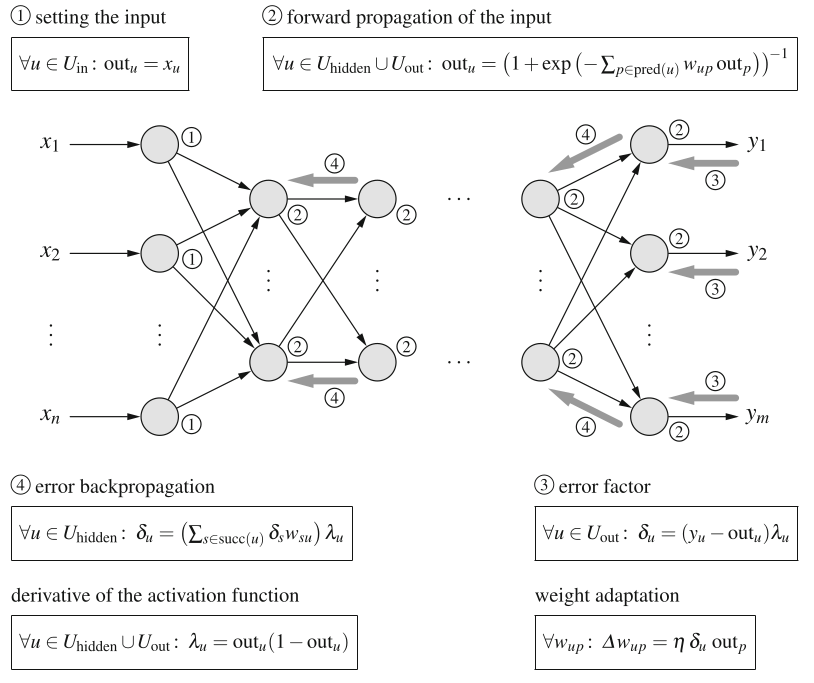
\includegraphics[scale=0.4]{img/backpropagation.png}
\caption{Propagazione dell'errore in un MLP.}
\label{fig:14}
\end{figure}

Inizialmente, (1) applichiamo l'input ai neuroni di input che lo restituiscono senza modifiche in output al primo dei layer hidden. (2) Calcoliamo per ogni neurone dei seguenti layer la somma pesata degli input e al risultato applichiamo la funzione logistica generando così l'output che verrà propagato in tutto il network fino ai neuroni terminali. A questo punto, (3) calcoliamo la differenza tra l'output atteso e quello attuale e, dato che la funzione di attivazione è invertibile, risaliamo dal vettore di errore a quale fosse l'input che ha condizionato quel particolare errore (la variabile $\delta_u$, nell'immagine). Avendo, ora, (4) trasformato l'errore della variabile di output $out_u$ in quello della variabile di input $net_u$ possiamo distribuire l'errore (e la correzione necessaria) in modo proporzionale al ruolo del singolo neurone nel calcolo del seguente output. Propago a ritroso l'errore fino ai neuroni di input. Bisogna osservare comunque che data la forma della funzione logistica l'errore non può sparire completamente, in quanto il gradiente approssimerà il vettore nullo più si avvicinerà allo zero. 

\begin{remark}
\emph{Se si inizializza il learning rate $\eta$ ad un valore troppo alto, al posto di discendere la curva si corre il rischio di saltare da un "picco" della funzione all'altro senza convergere mai al minimo. Inoltre, non è affatto detto che il minimo raggiunto in questo modo sia il minimo globale della funzione. La causa sarà piuttosto da ascrivere alla scelta dei valori iniziali. Una soluzione al problema può essere quella di ripetere l'apprendimento, inizializzando il sistema con una diversa configurazione di pesi e threshold, e scegliere alla fine quale configurazione risulta in un miglior minimo.}
\end{remark}

\subsubsection{Variazioni sul gradient descent}

Esistono varie sofisticazioni della tecnica del gradient descent che permettono un più veloce apprendimento e, nello stesso momento, un miglior controllo sulla lunghezza dei singoli step di apprendimento. Alcuni esempi sono:

\begin{itemize}
\item{\emph{Manhattan training}: utlizza al posto del valore del gradiente solo il suo segno per calcolare la direzione. Questo permette di semplificare notevolmente la computazione.}
\item{\emph{Flat spot elimination}: cerca di limitare l'abbattimento della lunghezza degli step di apprendimento quando ci si avvicina ad un plateau della funzione "sollevando" artificialmente la derivata della funzione in quel punto.}
\item{\emph{Momentum term}: ad ogni successivo step aggiungo al gradiente una frazione del precedente cambiamento di pesi così da avere una memoria di quanto velocemente stava cambiando nel passato.}
\item{\emph{Self-adaptive error backpropagation}: permetto ad ogni parametro di avere un diverso learning rate in modo da avere un più fine controllo rispetto alle caratteristiche del singolo parametro.}
\item{\emph{Resilient error backpropagation}: combina il Manhattan training con l'approccio self-adaptive.}
\item{\emph{Quick propagation}: al posto di utilizzare il gradiente approssimo la funzione con una parabola e salto direttamente all'apice della parabola.}
\item{\emph{Weight decay}: riduce i pesi per evitare di rimanere intrappolato in una regione già saturata.}
\end{itemize}

\subsubsection{Overfitting e underfitting}

Quanti neuroni ho bisogno per avere un buon network? Come regola di massima si dovrebbe scegliere il numero di neuroni negli hidden layer seconda la seguente formula:
$$
\# \text{hidden neurons} = (\# \text{input neurons} + \# \text{output neurons})/2
$$
Non esiste una spiegazione teoretica soddisfacente del perchè questo sia un buon numero, ma è stato dimostrato empiricamente. Se, infatti, il numero dei neuroni negli hidden layer è troppo basso rischiamo l'\emph{underfitting}, ossia che il nostro MLP non riesca ad approssimare in modo soddisfacibile la complessità della funzione che vogliamo catturare. Al contrario se ne ho troppi rischio di incorrere nell'\emph{overfitting}, ossia che il nostro MLP si adatti agli esempi che gli abbiamo fornito durante il periodo di apprendimento, ma anche alle loro specificità accidentali (errori e deviazioni).
Per evitare questi fenomeni è buona pratica dividere il nostro data set in modo da avere due sottoinsiemi di dati: alcuni dati per l'apprendimento ed altri per la validazione del processo di apprendimento. I primi verranno usati per allenare il nostro network e i secondi per giudicare se effettivamente il network approssimi la funzione desiderata. \'E possibile iterare a piacere questo procedimento suddividendo i dati non in due sottoinsiemi, ma in un numero arbitrario, così da ottenre una conferma incrociata dei progressi nell'apprendimento del nostro network.
Un diverso metodo per evitare l'overfitting è quello di terminare l'apprendimento quando il differenziale dell'errore tra un epoca ed un altra si abbassi sotto una certa soglia, oppure se l'apprendimento si protrae per un periodo troppo lungo.

\subsubsection{Sensitivity analysis}

Uno svantaggio delle ANN è che la conoscenza risultante dal processo di apprendimento è codificata in matrici a valori reali e, quindi, di difficile comprensione per l'utente. Abbiamo mostrato una interpretazione geometrica dei processi interni alle ANN, ma tale interpretazione, sebbene sia generalizzabile ad ANN arbitrariamente complesse, offre poco aiuto all'intuizione quando lo spazio degli input supera le tre dimensioni. Una soluzione a questo problema è quella di operare una \emph{sensitivity analysis}, la quale determinerà l'influenza dei vari input sull'output del network. Per eseguirla occorrerà calcolare la somma delle derivate parziali degli output rispetto agli input esterni per ogni neurone di output e ogni training pattern. Questa somma viene, infine, divisa per il numero di training pattern, per rendere la misura indipendente dalla grandezza del dataset.

$$
\forall u \in U_{(in)}: \quad s(u) = \frac{1}{|L|} \sum_{l \in L} \sum_{\nu \in U_{(out)}} \frac{\partial out_\nu^l}{\partial ext_u^l}
$$

Il valore $s(u)$ risultante indica quanto importante fosse l'input assegnato al neurone $u$ per la computazione del MLP. Grazie a questa considerazione potremmo decidere di semplificare il network eliminando i nodi con i valori di $s(u)$ più bassi.

\subsection{Deep learning}

Il Teorema 3 ha mostrato come un MLP con un solo hidden layer può approssimare ogni funzione continua su $\mathbb{R}^n$ con una precisione arbitraria. Questo risultato, tuttavia, non ha natura costruttiva e può non essere semplice conoscere a priori il numero esatto di neuroni necessari per approssimare una data funzione. Inoltre, a seconda della funzione, questo numero potrebbe assumere dimensioni considerevoli!
Un esempio è quello della funzione che calcola la parità su una parola di $n$-bit. L'output sarà 1 se e solo se nel vettore di input che rappresenta la parola saranno ad 1 un numero pari di bit. Nel caso scegliessimo di utilizzare un MLP con un solo hidden layer questo avrà al suo interno $2^{n-1}$ neuroni, in quanto la forma normale disgiuntiva della funzione di parità su $n$-bit è una disgiunzione di $2^{n-1}$ congiunzioni. 
Se permettiamo, invece, di avere più di un layer, il numero di neuroni crescerà in modo lineare alla dimensione dell'input. Questa constatazione ha portato allo sviluppo del così detto \emph{deep learning}, dove la "profondità" è quella del più lungo cammino che separa i neuroni di input da quelli di output. Il razionale è quello di permettere una maggiore profondità del network in cambio di un miglioramento delle risorse utilizzate nel calcolo e nella costruzione. Il deep learning oltre ad offrire vantaggi porta con se alcune problematiche:

\begin{itemize}
\item{\emph{Overfitting}: l'incremento nel numero di neuroni dovuto alla presenza dei molti layer può avere l'effetto di moltiplicare i parametri in modo sproporzionato.}
\item{\emph{Vanishing gradient}: durante la propagazione dell'errore il grandiente si riduce dopo ogni layer fino a scomparire.}
\end{itemize}

Alcune soluzioni al problema dell'overfitting sono:

\begin{itemize}
\item{\emph{Weigth decay}, ossia mettere un tetto massimo ai valori che possono assumere i pesi per prevenire un adattamento troppo pedissequo al dataset.}
\item{\emph{Sparsity constraint}: si introducono dei limiti al numero di neuroni negli hidden layer, oppure si limita il numero di quelli attivi.}
\item{\emph{Dropout training}: alcuni neuroni degli hidden layer vengono omessi durante l'evoluzione del network.}
\end{itemize}

\begin{figure}
\centering
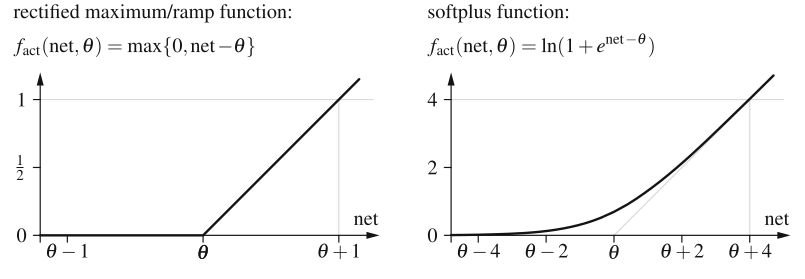
\includegraphics[scale=0.4]{img/relu.png}
\caption{Funzioni di attivazione sempre crescenti.}
\label{fig:15}
\end{figure}

Il problema del vanishing gradient è dato dal fatto che la funzione di attivazione è una funzione logistica la cui derivata raggiunge al massimo il valore di $\frac{1}{4}$. Di conseguenza, ogni propagazione dell'errore ad un layer precedente vi aggiunge un valore, spesso molto minore di 1, riducendo così il gradiente. Una soluzione è quella di modificare leggermente la funzione di attivazione in modo che sia sempre crescente. Alcuni candidati proposti in letteratura sono la \emph{ramp function} e la \emph{softplus function} (vedi Figura \ref{fig:15}).
Un approccio completamente diverso è quello di costruire il network "layer a layer". Una tecnica molto usata è quella di pensare al network come una pila di \emph{autoencoder}. Un autoencoder è un MLP che mappa il suo input in una sua approssimazione, utilizzando un hidden layer di dimensioni minori. Il layer nascosto funge da encoder per la codifica dell'input in una sua rappresentazione interna che è a sua volta decodificata dal layer di output. L'autoencoder, avendo un solo layer, non soffre delle stesse limitazioni e può essere allenato attraverso la normale backpropagation. Un problema con questo approccio è che se ci sono tanti neuroni negli hidden layer quanti quelli di input si rischia di propagare con minori aggiustamenti il segnale senza che l'autoencoder estragga alcuna informazione utile dal dato.
Esistono tre principali soluzioni:
\begin{itemize}
\item{\emph{Sparse autoencoder}: prevede di utilizzare un numero molto minore di neuroni nel hidden layer, rispetto a quelli di input. L'autoencoder sarà così costretto ad estrarre dall'input qualche feature interessante al posto di propagare semplicemente il dato.}
\item{\emph{Sparse activation scheme}: in modo simile a quanto si faceva per evitare l'overfitting, si decide di "spegnere" alcuni neuroni durante la computazione.}
\item{\emph{Denoising autoencoder}: si aggiunge randomicamente rumore all'input.}
\end{itemize}
Per ottenere un MLP con molteplici layer si combinano diversi autoencoder. Inizialmente si allena un singolo autoencoder. A quel punto, si rimuove il decoder e viene conservato solo il layer interno. Si utilizzano i dati preprocessati da questo primo autoencoder per allenarne un secondo, e così via fino a che si raggiunga un numero soddisfacente di layer.
MLP costruiti in questo modo sono risultati molto efficaci nel riconoscere con successo numeri scritti a mano. Se si volessero utilizzare dei network simili per una più ampia classe di applicazioni, dove, per esempio, le feature riconosciute dai layer interni non sono localizzate in una porzione specifica dell'immagine, bisognerebbe rivolgersi ai \emph{convolutional neural network} (più avanti, CNN). Questa architettura è ispirata al funzionamento della retina umana, in cui i neuroni adibiti alla percezione hanno un campo ricettivo, ossia una limitata regione in cui rispondono agli stimoli. Questo viene simulato nelle CNN connettendo i neuroni del primo hidden layer solo ad alcuni neuroni di input. I pesi vengono condivisi così che i vari network parziali possano essere valutati da differenti prospettive dell'immagine. Durante la computazione si procederà poi a muovere il "campo ricettivo" sulla totalità dell'immagine. Come risultato si ottiene una convoluzione della matrice dei pesi con l'immagine in input.

\subsection{Radial basis function network}

I così detti \emph{radial basis function network} (in quello che segue, RBFN) sono feed-forward network aventi tre layer di neuroni. Sono strutture alternative rispetto ai classici MLP. La differenza principale sta nella diversa scelta riguardo la funzione di attivazione. Se nel caso degli MLP avevamo una funzione sigmoide, ora avremo una funzione radiale di base \footnote{Una funzione radiale di base, o funzione di base radiale è una funzione a valori reali $f(x)$ il cui valore dipende unicamente tra la distanza dell'argomento $x$ e un punto prefissato $c$. Se il punto $c$ in questione è l'origine si dicono funzioni radiali.}. La $f_{net}$ dei neuroni di output è la somma pesata dei loro input, come in precedenza. Invece, per i neuroni nel hidden layer avremo che $f_{net}$ sarà uguale alla distanza tra il vettore di input e il vettore dei pesi. La funzione distanza che sceglieremo sarà una metrica in senso geometrico, e, per tanto, deve rispettare i seguenti tre assiomi:
$$
d(\ww,\vv) = 0 \leftrightarrow \ww = \vv
$$
$$
d(\ww,\vv) = d(\vv,\ww)
$$
$$
d(\ww,\ee) + d(\ee,\vv) \geq d(\ww,\vv)
$$
Una famiglia di funzioni usate spesso nelle applicazioni è quella formulata dal matematico prussiano Hermann Minkowski e battezzata in suo onore famiglia di Minkowski. Tale famiglia è definita come:
$$
d(\ww,\vv)_k = (\sum (w_i - v_i)^k)^{\frac{1}{k}}
$$
Alcuni esempi famosi di funzioni appartenenti alla famiglia sono:
$$
k = 1: \text{Manhattan distance}
$$
$$
k=2:\text{Euclidian distance}
$$
$$
k = \infty: \text{Maximum distance, ovvero } d(\ww,\vv)_\infty = max |w_i - v_i|
$$
\begin{figure}
\centering
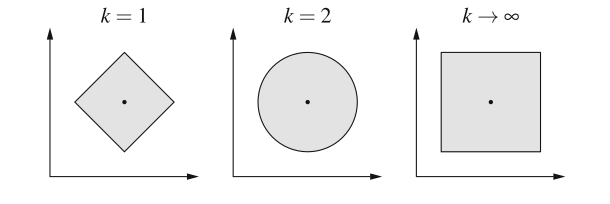
\includegraphics[scale=0.4]{img/circle.png}
\caption{Cerchi rispetto alle diverse definizioni di distanza.}
\label{fig:16}
\end{figure}
Un modo utile di visualizzare queste funzioni è quello di vedere che forma assume un cerchio a seconda delle varie metriche (vedi Figura \ref{fig:16}). La ragione è che un cerchio è definito come quell'insieme di punti che stanno alla stessa distanza da un dato punto. Variando la definizione di distanza, varia la forma che assume il cerchio nei diversi spazi.
Passando ora a considerare $f_{act}$ avremo, nel caso dei neuroni di output, una funzione lineare. Invece, per i neuroni del hidden layer avremo una funzione monotona decrescente tale che:
$$
f: \mathbb{R}^{+} \to [0,1] \quad \text{con} \quad f(0) = 1 \quad \text{e} \quad \lim_{x \to \infty} f(x) = 0
$$
Questa funzione calcola l'area in cui il neurone focalizza la propria attenzione definita dal raggio di riferimento $\sigma$. I vari parametri e la forma della funzione determinano l'ampiezza di questa area. Le funzioni più utilizzate per determinare l'area di attivazione sono quelle riportate in Figura \ref{fig:17}.
\begin{figure}
\centering
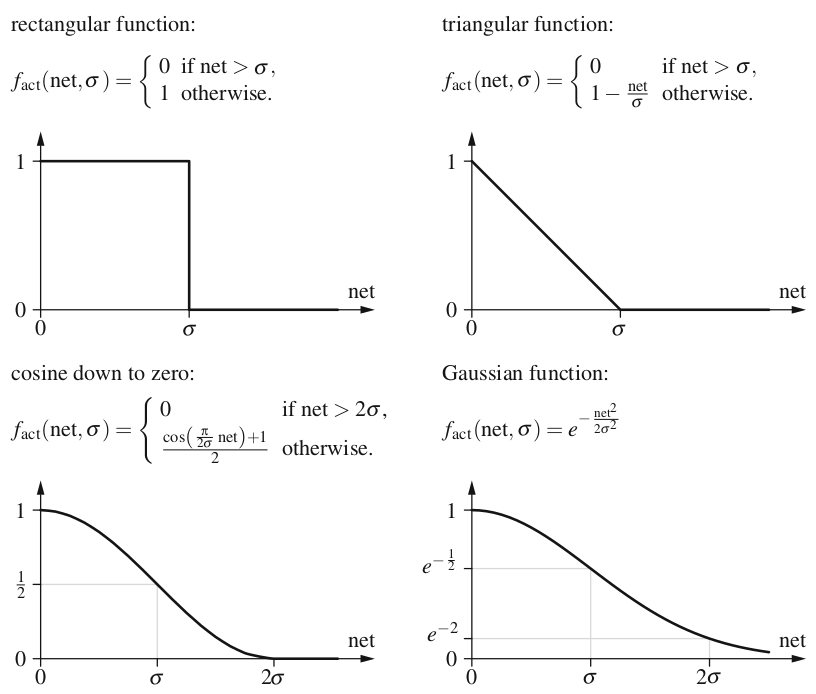
\includegraphics[scale=0.3]{img/act_rbf.png}
\caption{Varie funzioni di attivazione per un RBFN.}
\label{fig:17}
\end{figure}
Come esempio, applichiamo un RBFN per simulare una congiunzione booleana. Un network che risolve il problema è quello costituito da un singolo neurone hidden, il cui vettore dei pesi (il centro della funzione radiale) è esattamente il punto in cui in output vorremo il valore \emph{vero}, ovvero (1,1). Il raggio $\sigma$ sarà posto a $\frac{1}{2}$ e verrà codificato nel threshold del neurone. La funzione di distanza usata è quella euclidea e come $f_{act}$ utilizziamo una funzione rettangolare. Il diagramma in Figura \ref{fig:18} offre una rappresentazione grafica di quanto detto. 
\begin{figure}
\centering
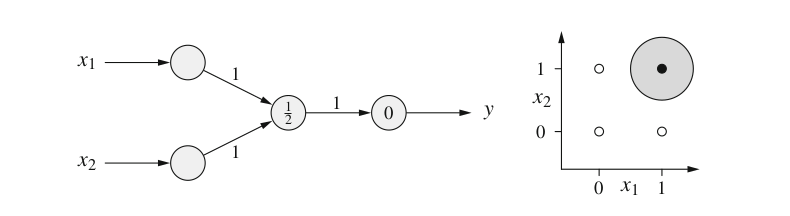
\includegraphics[scale=0.4]{img/and_rbf.png}
\caption{RBFN che calcola la congiunzione booleana.}
\label{fig:18}
\end{figure}
In generale, un RBFN ha lo stesso potere espressivo di un MLP e può essere visto come un approssimatore universale, ovvero può approssimare (con errore arbitrariamente piccolo) una qualsiasi funzioni Riemann-integrabile. Il procedimento è lo stesso che nel caso degli altri network: la funzione viene approssimata da una funzione a scalini che può essere calcolata facilmente da una funzione radiale se la definiamo come la somma pesata di funzioni rettangolari. L'approssimazione può essere migliorata aumentando il numero dei punti in cui si valuta la funzione. Inoltre, se al posto della funzione rettangolare, viene utilizzata una funzione Gaussiana possiamo ottenere delle transizioni più "morbide" evitando bruschi salti. 

\subsection{Training delle RBFN}

Se negli altri ANN la fase di inizializzazione era triviale, in quanto bastava scegliere valori in modo casuale, quando si tratta di RBFN lo stesso approccio conduce a risultati subottimali. Consideriamo, quindi, il caso speciale delle \emph{simple radial basis function network}, dove ogni esempio di apprendimento viene associato ad una propria funzione radiale. Dato un fixed learning task $L = \{l_1,\dots,l_m\}$, avente $m$ pattern $l = (\ii^l,\oo^l)$, definiremo il vettore dei pesi associato al neurone $v_k$ come:

$$
\forall k \in \{1,\dots,m\}: \ww_{v_k} = \ii_k
$$

Assumendo una funzione di attivazione gaussiana, il raggio $\sigma_k$ è inizializzato in accordo a questa euristica:

$$
\forall k \in \{1,\dots,m\}: \sigma_k = \frac{d_{max}}{\sqrt{2m}}
$$

Dove $d_{max}$ è la massima distanza tra i vettori di input. Questa scelta permette di centrare le varie gaussiane in modo che non si sovrappongano l'una all'altra, ma si distribuiscano in modo ordinato rispetto allo spazio di input. Per quanto riguarda, invece, i pesi dei neuroni di output, vengono calcolati secondo la seguente funzione:
$$
\forall u: \sum_{k=1}^m w_{u_k} out_{u_k} - \theta  = o_u
$$
Ponendo $\theta = 0$, avremo che la precedente equazione è equivalente a:
$$ 
\mathbf{A}\cdot \ww_u = \oo_u
$$
Dove $\mathbf{A}$ è la matrice $m \times m$ che ha come componenti i vari output dei neuroni nel hidden layer. Se la matrice $\mathbf{A}$ ha rango completo, possiamo invertirla e calcolare il vettore dei pesi come segue:
$$
\ww_u = \mathbf{A}^{-1}\cdot \oo_u
$$
Questo metodo garantisce una perfetta approssimazione. Non è necessario, quindi, allenare un simple radial basis function network. In generale, se non vogliamo avere per ogni training pattern un neurone, dovremo selezionare $k$ sottoinsiemi del dataset e trovare, per ogni sottoinsieme, un rappresentante che  assoceremo ad un neurone nel layer hidden. In analogia a quanto accade nel caso "semplice" avremo una matrice $\mathbf{A}$ di dimensione $m\times (k+1)$ con i valori in output dei vari neuroni nel hidden layer. Dato che la matrice non è quadrata, non è possibile calcolarne l'inversa come avevamo fatto in precedenza. Tuttavia, esiste una alternativa chiamata la \emph{matrice pseudo-inversa}\footnote{La matrice pseudo-inversa $\mathbf{A}^+$ della matrice $\mathbf{A}$ è calcolata come $\mathbf{A}^+ = (\mathbf{A}^{\top}\mathbf{A})^{-1}\mathbf{A}^{\top}$} che permette di completare il calcolo con una buona approssimazione. Ovviamente, l'accuratezza del network costruito in questo modo dipenderà dalla precisione con cui si scelgano i rappresentati delle varie sottoclassi del dataset. Esistono vari metodi per fare questo:
\begin{itemize}
\item{Scegliamo tutti i punti del dataset come centri. In questo caso ricadiamo nel caso "semplice" e i valori di output possono essere calcolati precisamente. Tuttavia, il calcolo dei pesi può risultare infattibile.}
\item{Costruiamo un sottoinsieme randomico per rappresentare i centri. Questo metodo ha il pregio di essere facilmente calcolabile. La performance, però, dipenderà dalla fortuna di scegliere dei "buoni" centri.}
\item{Utilizziamo un algoritmo di clustering (c-means clustering,learning vector quantization..)}
\end{itemize}


\begin{remark}
\emph{L'algoritmo c-means sceglie randomicamente $c$ centri di altrettanti cluster. Quindi il dataset viene partizionato in $c$ sottoclassi a seconda della vicinanza ai vari centri. In un passo successivo si calcola il "centro di gravità" del cluster così trovato e lo si elegge come nuovo centro. Si ricomputa l'appartenza dei punti del dataset e si procede così fino a che i centri smettono di oscillare.}
\end{remark}

La fase di training avviene come nel caso dei MLP attraverso il gradient descent e la backpropagation. 
\section{Sistemi fuzzy}


\section{Algoritmi evolutivi}


\end{document}